\chapter{Introduction and Case Background}
\label{ch:intro}

\section{Context and motivation}

Language-model agents now operate software for people. They open web pages, fill in forms, click buttons and read results~\cite{zhou2024webarena,he2024webvoyager,xie2024osworld}. Many such agents send each observation, often a screenshot of a logged-in page, to a hosted multimodal model~\cite{he2024webvoyager,zheng2024seeact,zhang2025ufo}. Those screens carry names, messages and account data, which the hosted provider then processes and may retain, and language models can leak personal information they were trained on~\cite{lukas2023pii}.

A second problem is less visible. An agent can stop too early. I call this \emph{premature completion}: the agent reports ``done'' while the page does not satisfy the goal. A typical case is an agent that opens the search engine, types nothing, and declares the search finished. Each action succeeded; the task did not. In most agent frameworks the language model itself decides when a task is finished~\cite{yao2023react,shinn2023reflexion}, and studies show that a model correcting itself without outside feedback does not reliably improve~\cite{huang2024cannot}.

These two problems meet in one question that this case study tries to answer from evidence: can an agent that keeps its data on the user's machine also refuse to claim success until the screen shows it, and what does that refusal cost? Fig.~\ref{fig:conv-vs-gate} contrasts a conventional agent loop with the evidence-gated loop examined in this case.

\begin{figure}[h]
\centering
\begin{tikzpicture}[font=\footnotesize,
  box/.style={draw,rounded corners=2pt,minimum height=0.85cm,text width=2.25cm,align=center},
  gate/.style={box,fill=blue!10,draw=blue!60!black},
  arr/.style={-{Stealth[length=2mm]}}]
\node[font=\small\bfseries,anchor=west] at (-1.3,1.0) {(a) Conventional agent loop};
\node[box] (a1) at (0,0) {Goal $g$};
\node[box,right=0.45cm of a1] (a2) {Model plans action $a_t$};
\node[box,right=0.45cm of a2] (a3) {Execute; dispatch flag $\alpha_t$};
\node[box,right=0.45cm of a3] (a4) {Model says ``done''};
\draw[arr] (a1)--(a2); \draw[arr] (a2)--(a3); \draw[arr] (a3)--(a4);
\draw[arr] (a3.south) -- ++(0,-0.35) -| (a2.south);
\node[font=\small\bfseries,anchor=west] at (-1.3,-1.6) {(b) Evidence-gated loop in Agentic Pilot};
\node[box] (b1) at (0,-2.6) {Goal $g$, plan $P$ (local model)};
\node[box,right=0.45cm of b1] (b2) {Execute in Chromium; observe $s_{t+1}$};
\node[gate,right=0.45cm of b2] (b3) {Completion gate $\Phi(g,s_{t+1},P)$};
\node[gate,right=0.9cm of b3] (b4) {Report done + store evidence};
\draw[arr] (b1)--(b2); \draw[arr] (b2)--(b3); \draw[arr] (b3)--node[above,font=\scriptsize]{holds}(b4);
\draw[arr] (b3.south) -- ++(0,-0.4) -| node[pos=0.25,below,font=\scriptsize]{fails: continue or re-plan} (b1.south);
\end{tikzpicture}
\caption{A conventional agent loop (a) and the evidence-gated loop examined in this case (b). Shaded steps do not exist in (a).}
\label{fig:conv-vs-gate}
\end{figure}

\section{Description of the case}

\subsection{Organisation and setting}
The case is the Agentic Pilot prototype, which I built as an M.Tech student in the Department of Computing Technologies, SRM Institute of Science and Technology, Kattankulathur, under the guidance of Dr. Kanchana M. Its main written record is the research paper ``Agentic Pilot: An Evidence-Driven Local Autonomous AI Agent Framework for Privacy-Preserving Intelligent Task Automation''. The code, data and scripts are public under the MIT licence at \url{https://github.com/sudeshsudhii/Agentic-pilot-local}; the evaluated agent code is commit \texttt{bf0a8a5} on branch \texttt{ccr-4b8200f0-5i3k5m}. Every number in this report can be traced to a file on that branch.

\subsection{Domain}
The domain is task automation in a web browser by an AI agent: searching, opening pages, entering text, extracting facts and completing short multi-step tasks for a user who types a request in plain language. The agent acts only in a Chromium browser. It is \emph{autonomous} in that, given a request, it plans and executes browser actions without step-by-step instructions; the user approves tasks classified as high-risk (posting, sending, purchasing, deleting, transferring) and solves CAPTCHAs. It is \emph{privacy-preserving} in a narrow sense: by default its model client sends prompts and screenshots only to a model server on the loopback interface, and it writes task records, memory and evidence only to local files.

\subsection{Technology}
The backend is written in Python (about 11{,}000 lines) on FastAPI, LangGraph, Playwright and Pydantic, with SQLite for task events and a persistent local Chroma store for memory. Model calls use the Ollama HTTP API with JSON output. A router assigns each call one of the installed local Qwen2.5, Qwen3.5 or DeepSeek-R1 models (1.5B to 7B parameters) or a small vision model. The client is React in a Tauri desktop shell. Fig.~\ref{fig:arch} shows the architecture.

\begin{figure}[h]
\centering
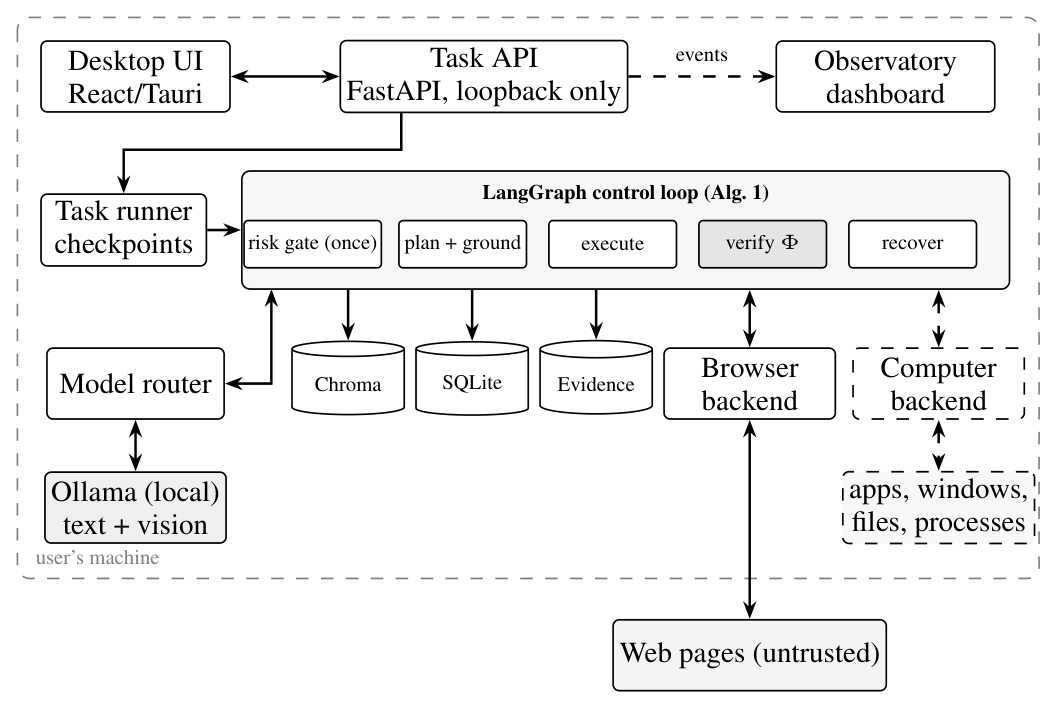
\includegraphics[width=0.95\textwidth]{fig/architecture.png}
\caption{Architecture of Agentic Pilot: desktop client, loopback FastAPI service, LangGraph control loop with the completion gate, Playwright browser backend, local models and local stores}
\label{fig:arch}
\end{figure}

The control loop is a compiled LangGraph state machine with eleven nodes. A typed state record carries the intent, the plan and step index, the current observation, the planned action, the action history, retry and model-call counters and the status. Only the verification node can end a task as \textsc{Completed}, and only when the completion predicate $\Phi$ holds. Each observation lists up to 50 ranked interactable page elements with role, label, text and selectors, sanitised against prompt injection. Actions are navigate, click, type, key press, scroll and extract; typed text is read back from the page. For each task, an evidence directory holds before-and-after screenshots of each action, the latest DOM manifest, the verification and recovery records and the node trace.

\subsection{Stakeholders}
Table~\ref{tab:stake} lists the groups the design has to keep in mind and what each needs from the system.

\begin{table}[h]
\caption{Stakeholders of the case and what each needs}
\label{tab:stake}
\small\singlespacing
\begin{tabularx}{\textwidth}{|p{3.3cm}|L|L|}
\hline\hrow \textbf{Stakeholder} & \textbf{Role in the case} & \textbf{What they need from the system}\\\hline
End users & Type requests and approve risky actions & Tasks done correctly; an honest ``not done''; screens not sent off the machine\\\hline
Developer (the author) & Designed, built and evaluated the prototype & Reproducible runs and records that support each claim\\\hline
Guide and examiners & Supervise and assess the work & Claims that match the evidence; clear separation of measured and simulated results\\\hline
Model publishers & Release open-weight models (Qwen, DeepSeek) run through Ollama & Correct use within licence terms\\\hline
Website operators & Run the sites the agent visits & No CAPTCHA solving or bot-check evasion by the agent\\\hline
Regulators and the institution & Set rules on personal data and software & Personal data kept on the device; compliance with the DPDP Act, 2023\\\hline
\end{tabularx}
\end{table}

\section{Problem statement and research questions}

A conventional agent equates a successful action call with progress and lets its model decide when the task is over. The problem in this case is to design an agent that keeps its inference and records on the user's machine, separates \emph{action dispatch} from \emph{task completion}, reports completion only when the observed page supports it, and to measure what this achieves and costs without overclaiming.

The research paper states three gaps, each phrased so that it can be tested:
\begin{itemize}
\item \textbf{G1.} In-loop completion checks are rarely measured. Does a rule over observed state inside the loop withhold premature completions, and at what false-rejection cost, on held-out data?
\item \textbf{G2.} The contribution of each kind of evidence is unknown. Does removing a conjunct of the rule raise false completions?
\item \textbf{G3.} Locality claims of local agents are rarely checked. Does the agent's process contact any host other than the local machine?
\end{itemize}
Five hypotheses, H1 to H5, extend these questions to the whole agent: fewer false completions (H1), more reliable completion decisions (H2), the effect of memory (H3), the effect of the recovery engine (H4) and the time overhead of verification (H5). They are examined in a seeded simulation, because a full study with a language-model planner was outside the scope of this case.

\section{Objectives and scope of the study}

The objectives are:
\begin{itemize}
\item to describe the prototype, its stakeholders and its setting well enough for the design to be judged;
\item to review related work on reasoning-and-acting agents, web and computer-use agents, completion checking, memory, security and local inference;
\item to analyse the recorded evidence with suitable statistics, tracing every number to a run record;
\item to compare what theory predicts with what the system did; and
\item to recommend how the work should proceed, with alternatives, risks and measures of success.
\end{itemize}

The study covers the browser backend and its components: the completion gate, browser control, locality enforcement, memory retrieval, recovery classification and the end-to-end oracle. Task-level success of the full agent with a language-model planner, the desktop backend (designed but not implemented in the evaluated commit) and physical hardware are out of scope.

\section{Different viewpoints on the case}
Table~\ref{tab:views} summarises five viewpoints on the prototype.

\begin{table}[h]
\caption{Summary of viewpoints on the case}
\label{tab:views}
\small\singlespacing
\begin{tabularx}{\textwidth}{|p{2.2cm}|L|L|}
\hline\hrow \textbf{Viewpoint} & \textbf{Main concern} & \textbf{What the case shows}\\\hline
Technical & Does the gate catch premature claims, and at what cost? & Withholds 9 of 22 held-out unsatisfied states, rejects 1 of 20 satisfied; 27\,ms per decision\\\hline
User and business & Is the agent useful if it sometimes refuses? & An honest ``not done'' is cheaper than a false ``done''; the gate's checks cover only some phrasings\\\hline
Social & Does it reduce misplaced trust in AI agents? & Stored evidence lets a user see why a task was or was not reported complete\\\hline
Ethical & Is the evaluation honest about what was measured? & Every number carries an evidence class; simulated results are not presented as measurements\\\hline
Legal & Is personal data handled lawfully? & Screens and prompts stay on the machine by default, which supports data minimisation under the DPDP Act, 2023\\\hline
\end{tabularx}
\end{table}

\textbf{Technical viewpoint.} A completion claim is accepted only when every check that the request triggers agrees. The measured cost is a median of 26.8\,ms per decision and no model call.

\textbf{User viewpoint.} A refused claim sends the agent back to work or ends the task honestly as unfinished. The user loses some convenience but gains a report they can trust.

\textbf{Social and ethical viewpoint.} Agents that overstate success can mislead people into acting on work that was never done. The evidence records make each decision inspectable.

\textbf{Legal viewpoint.} India's Digital Personal Data Protection Act, 2023 asks that personal data be processed for a lawful purpose and kept to what is necessary. An agent whose model runs on the user's own machine avoids transferring screen contents to a third party by default.

\section{Organisation of the report}
Chapter~\ref{ch:lit} reviews sources and related work. Chapter~\ref{ch:analysis} analyses the evidence and its limits. Chapter~\ref{ch:theory} applies the underlying theory. Chapter~\ref{ch:insights} draws insights and recommends a way forward, and Chapter~\ref{ch:concl} concludes. The appendices hold code listings, configuration, data samples and the run records.
